\documentclass[preprint,10pt,authoryear]{elsarticle}
\usepackage{graphicx} 
\usepackage{amssymb}
\usepackage{amsmath}
\usepackage{float}
\usepackage{array}
\usepackage{booktabs}
\usepackage{subcaption}
\begin{document}

\begin{frontmatter}

\title{Is the Phillips Curve still Alive? Panel Evidence from Founding Eurozone Members}
\author{Dominykas Vaičiūnas, Anabela Vaitkevičiūtė, Oskaras Rodionov, Kipras Petruitis}


\end{frontmatter}

\section{Introduction}

The relation between inflation and unemployment was always important  to analyze both for policy implications and theoretical interest. It was A.W.Phillips who found a negative relation between the two in the UK in 1958. The theory soon became known as the Phillips Curve. It was then expanded by other economists who added Non Accelerating Inflation Rate of Unemployment and inflation expectations to the Phillips curve analysis (Friedman, 1968). Of course, such topic is very important for policy questions since negative relation implies that governments have to balance between both even though neither of them being high is preferable. Of course what was found almost 70 years ago does not have to hold in recent times. Many papers since found that Phillips Curve is changing in magnitude even though the negative relation remained (Blanchard, 2015), (Ball, 2021). Particularly, the altering happened after various economic crises such as 1970s Energy Crisis or 2008-09 Great Recession. On top of that, as the world has changed due to globalization, it is inevitable that the Phillips Curve needs to be constantly rechecked to see if it has run out of steam.

We contribute to this literature by analyzing ten founding Eurozone members (Austria, Belgium, Finland, France, Germany, Ireland, Italy, the Netherlands, Portugal, and Spain) - countries sharing ECB monetary policy yet heterogeneous in labour markets and institutions, making them a more interesting case than the US-focused literature. Our sample runs from 1999Q1 to 2019Q4 using quarterly data, excluding the Covid period. We identify 2008–2009 as the crisis period based on GDP growth, forming two subsamples (1999–2007 and 2010–2019) to test whether the Phillips Curve changed after the crisis. Data used is from FRED and OECD.

We estimate four progressively augmented Two-way fixed effects models, ranging from a simple unemployment specification to an expectations-augmented Phillips curve. 

Then we form the hypotheses given the previous research for this topic: 1) There is a negative relationship between inflation and unemployment which is consistent with the Phillips Curve. 2) Period after 2008-2009 financial crisis has a weaker relation between inflation and unemployment than the period before. 3) More complex models we introduce are better at explaining the relation between inflation and unemployment, especially for period after the financial crisis.

Our results support the hypotheses. We find a  statistically significant negative relation between unemployment and inflation in the full sample which is consistent with Hazell et al. (2022) and Ball and Mazumder (2019). Subsample analysis shows that the Phillips Curve flattened after the crisis. Finally, more complex models show consistently steeper Phillips Curve and explain more variation of the inflation but we cannot be truly sure that they explain the actual relation better due to various introduced biases in the process.

The remainder of this report is structured as follows. Section 2 reviews the relevant literature. Section 3 states our hypotheses. Section 4 describes the methodology and regression specifications. Section 5 presents the data and reports summary statistics. Section 6 analyses correlations between inflation and unemployment across countries and periods. Section 7 presents and discusses the regression results. Section 8 concludes.

\section{Literature review}

This literature review examines theoretical and empirical research on the Phillips Curve, with particular attention to its applicability in the Eurozone economies in modern times. The original Phillips Curve was a concept indicating a negative relationship between unemployment rate and inflation (Phillips, 1958). Subsequent Phillips Curve literature developed into two major approaches: the expectations-augmented Phillips Curve and the New Keynesian Phillips Curve (R.J. Gordon, 2011), (M. Del Negro, M. L. Giorgio, E. Primiceri, A. Tambalotti, 2020). The expectations-augmented Phillips curve introduced concepts such as NAIRU and adaptive inflation expectations (J. Hazell, J. Herreno, E. Nakamura, J. Steinsson, 2022). The same paper also presents the New Keynesian Phillips curve theory, introducing concepts such as forward-looking inflation expectations (J. Hazell, J. Herreno, E. Nakamura, J. Steinsson, 2022).
Subsequently, we have looked into the empirical findings. Recent empirical studies suggest that the Phillips Curve relationship has weakened in advanced economies over time (L. Ball, S. Mazumder, 2019). While existing literature examines the Phillips Curve in both OECD and Eurozone contexts, fewer studies focus specifically on the 11 founding Eurozone members across our proposed period.

\section{Hypotheses}
The main hypothesis: There is a negative relationship between inflation and unemployment in the founding Eurozone countries which is consistent with the Phillips Curve.

Additional hypothesis: Period after 2008-2009 financial crisis has a weaker relation between inflation and unemployment than the period before. Expectations adjusted with NAIRU Phillips curve is better at explaining the relation between inflation and unemployment, especially after the financial crisis.

\section{Methodology}
In this report, we take the most important theoretical models for the Phillips curve and apply them to four distinct Two-way fixed effects regressions. Two way fixed effects regression excludes time-invariant effects from the regression (like institutional structure, inflation preferences, average productivity level). We also remove time variant effects that affect all countries (Global financial crisis, oil price shocks, ECB monetary policy). We are estimating within-country, over-time deviation from the common trend. This helps our analysis because we need fewer control variables to tackle omitted variable bias. To control for both serial correlation within countries over time and cross-sectional dependence across countries within periods, we report two-way clustered standard errors, clustering simultaneously by country and quarter (Cameron, 2011).

The first regression $\pi_{it,q} = \beta \cdot u_{it,q} + \mu_{i} + \lambda_{t,q} + \varepsilon_{it,q}$, is the simplest and most faithful to original concept of the Phillips curve (Phillips, 1958).

The second regression: $\pi_{it,q} = \beta \cdot u_{it,q} + \delta \cdot X_{it,q} + \mu_{i} + \lambda_{t,q} + \varepsilon_{it,q}$, we include two control variables that we think are important for fixed effects regresssion: Trade union density and Globalization rating. We believe that these variables will capture unit-specific time-varying confounders which are by contruction left over in two-way fixed effects regression.

Third regression: $\pi_{it,q} = \beta \cdot (u_{it,q} - u^{*}_{it,q}) + \delta \cdot X_{it,q} + \mu_{i} + \lambda_{t,q} + \varepsilon_{it,q}$, includes NAIRU and constructs an unemployment gap. We use simple HP filter (with frequency of 1600 because our data is quarterly) to contruct NAIRU due to lack of data available for our specific time and country dataset. This model is the most consistent with the actual theoretical idea of the Phillips curve where NAIRU is the explanatory variable of inflation (Friedman, 1968).

The fourth regression: $\pi_{it,q} = \gamma \cdot \pi^{e}_{it,q} + \beta \cdot (u_{it,q} - u^{*}_{it,q}) + \delta \cdot X_{it,q} + \mu_{i} + \lambda_{t,q} + \varepsilon_{it,q}$ adds inflation expectations. This model is sometimes called expectations-augmented Phillips curve and is widely used in more contemporary research (Roberts, 1995). We use a very simplified method: lagged inflation by one year as a proxy to capture these inflation expectations (Galí, 1999).


\section{Data}
We use our own constructed data set which includes data mostly from FRED. Our countries of interest are the ten founding members of Eurozone and the time frame is from 1999-2019. All variables are quarterly to have more observations for more credible analysis. 

Inflation is constructed using FRED data on CPI for all prices expect food and energy. We believe this will help to make the analysis more credible. This is because we do not need to control for energy supply shocks in our regressions and the data is less susceptible to big fluctuations. Unemployment is measured in percent from FRED for 15 years or older individuals and seasonally adjusted to control for unemployment that is seasonal and not of interest for our analysis. Trade union density is from OECD dataset as percentage of employees in the trade unions at that specific time. Globalisation rating is constructed using KOF Globalisation Index from 0 to 100 where higher number means more globalised. As a result, we have a panel data structure.

We also analyze which period to define as financial crisis in our dataset. We provide our own constructed average GDP growth graph for the chosen 10 countries which shows that the lowest growth was in 2008 and 2009. This is why in our analysis we not only analyze full 1999-2019 sample but also 1999-2007 and 2010-2019 subsamples to check our additional hypothesis whether Phillips Curve flattened after the crisis. Subsample excluding just 2008 and 2009 is also included to check robustness of the results of the full sample.  


\begin{figure}[H]
\centering
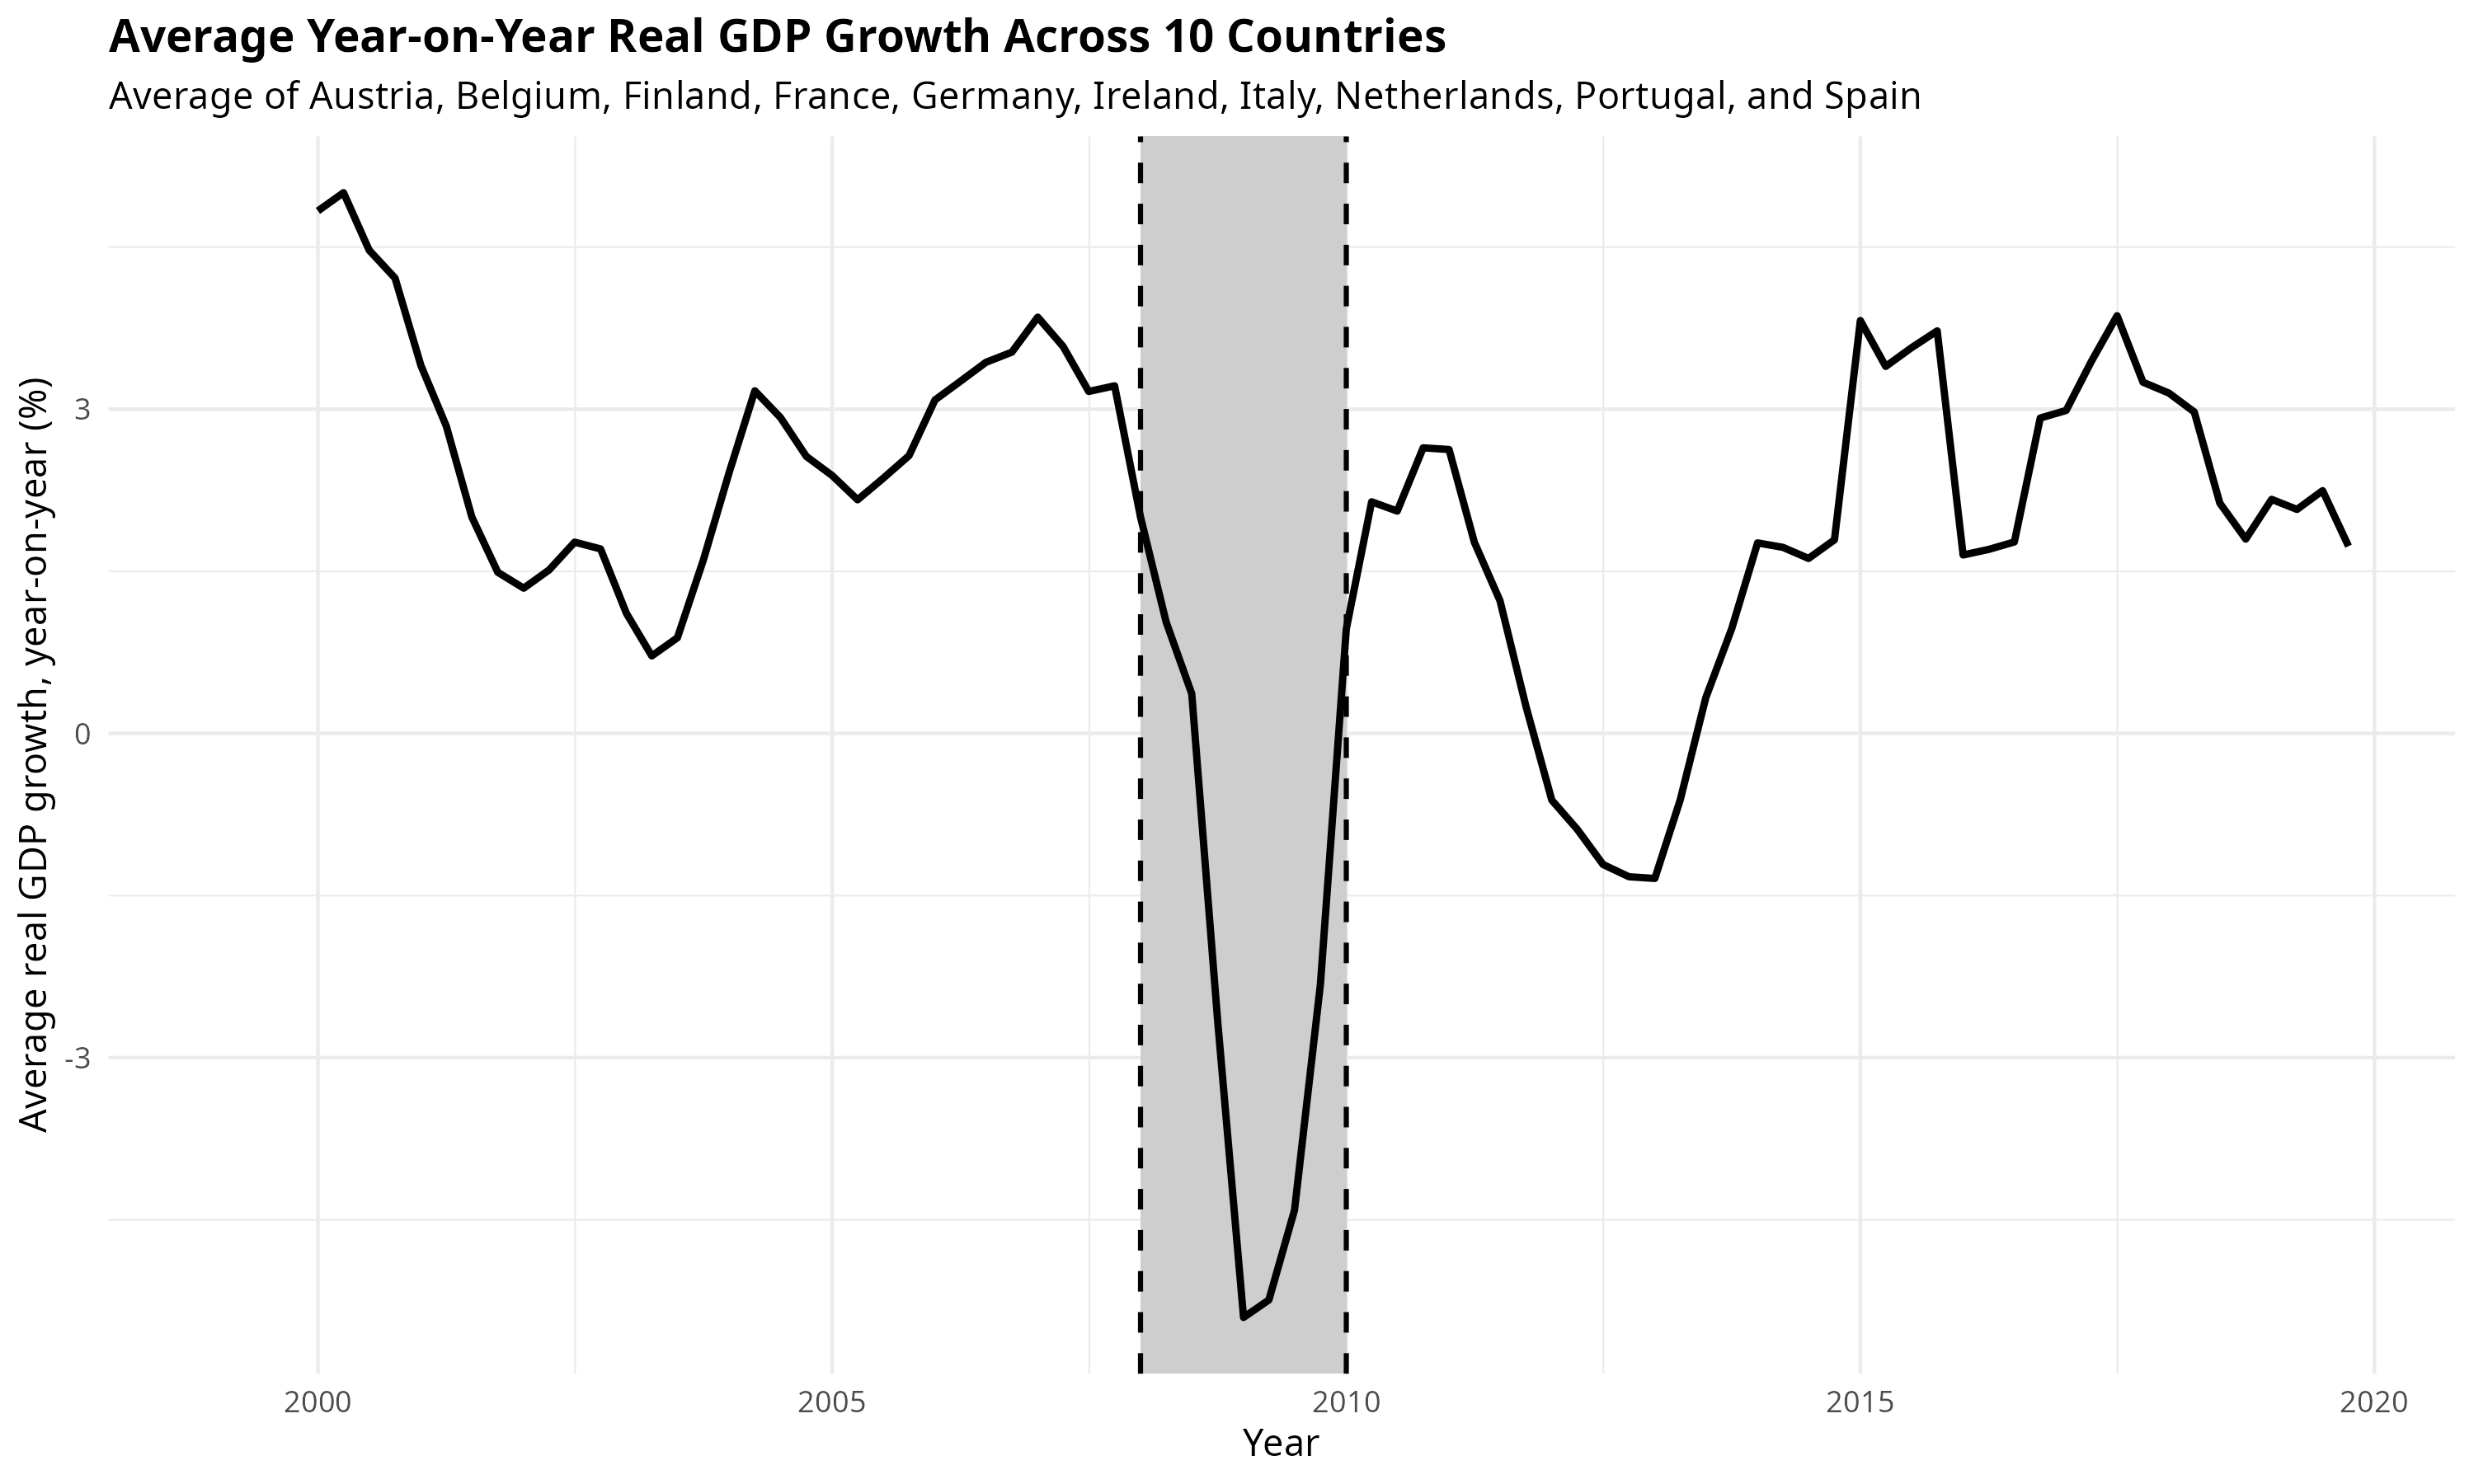
\includegraphics[width=0.8\textwidth]{average_gdp_growth_chart.png}
\caption{Average Year-on-Year real GDP growth across 10 countries}
\label{fig:gdp}
\end{figure}


\begin{table}[H] \centering 
  \caption{Summary table for the main statistics} 
  \label{} 

\begin{tabular}{@{\extracolsep{5pt}} cccccc} 
\\[-1.8ex]\hline 
\hline \\[-1.8ex] 
Variable & N & Mean & SD & Min & Max \\ 
\hline \\[-1.8ex] 
Inflation & 840 & 1.6 & 1.16 & -5.7 & 6.75 \\ 
Unemployment & 840 & 8.58 & 3.94 & 2.9 & 26.3 \\ 
\hline \\[-1.8ex] 
\end{tabular} 

\end{table} 




\begin{table}[H] \centering 
  \caption{Summary table for the main statistics by country} 
  \label{} 
   \resizebox{\textwidth}{!}{
\begin{tabular}{@{\extracolsep{5pt}} ccccccccc} 
\\[-1.8ex]\hline 
\hline \\[-1.8ex] 
 & Inf\_Mean & Inf\_SD & Inf\_Min & Inf\_Max & U\_Mean & U\_SD & U\_Min & U\_Max \\ 
\hline \\[-1.8ex] 
Austria & $1.860$ & $0.820$ & $0.030$ & $3.730$ & $5.220$ & $0.770$ & $3.630$ & $6.630$ \\ 
Belgium & $1.680$ & $0.410$ & $0.300$ & $2.710$ & $7.640$ & $0.950$ & $5.170$ & $8.970$ \\ 
Finland & $1.290$ & $0.920$ & $$-$0.690$ & $3.080$ & $8.400$ & $1.010$ & $6.170$ & $10.600$ \\ 
France & $1.130$ & $0.550$ & $0.280$ & $2.460$ & $9.150$ & $0.840$ & $7.100$ & $10.730$ \\ 
Germany & $1.160$ & $0.430$ & $0.350$ & $2.070$ & $6.770$ & $2.480$ & $2.900$ & $11.200$ \\ 
Ireland & $1.950$ & $2.580$ & $$-$5.700$ & $6.750$ & $8.080$ & $4.080$ & $3.900$ & $15.930$ \\ 
Italy & $1.580$ & $0.720$ & $0.370$ & $2.850$ & $9.500$ & $1.930$ & $6$ & $12.900$ \\ 
Netherlands & $1.750$ & $0.780$ & $0.240$ & $3.800$ & $5.790$ & $1.490$ & $3.100$ & $8.670$ \\ 
Portugal & $1.910$ & $1.290$ & $$-$0.150$ & $5.090$ & $9.530$ & $3.990$ & $3.930$ & $18.450$ \\ 
Spain & $1.730$ & $1.060$ & $$-$0.220$ & $3.660$ & $15.710$ & $5.660$ & $7.970$ & $26.300$ \\ 
\hline \\[-1.8ex] 
\end{tabular} 
}
\end{table} 

Countries’ quarterly inflation mean is close to 2\%, close to European Central bank goal. Only France, Finland and Germany, whose inflation mean is closer to 1\%. German consistently low inflation can be explained by Hartz reforms that expanded low-wage sector, fuelling wage stagnation that does not let inflation spiral; Fiscal policy is done to avoid large deficits and stick to balanced budgets by lower public investment; Anchored expectations of lower inflation lower inflation (revelatory!) 

The standard deviation of inflation is not-much-volatile in most of sampled countries, being less than 1, slightly more in Spain and Portugal and much more in Ireland (In Ireland volatility is around 2.5. Biggest part of this volatility can be explained by presence of multinational companies that swing GDP and price metrics based on global corporate activity).  

Lowest inflation for most countries was close to zero, some deflation happening. Ireland was exception in this metric again with lowed inflation being -5.7 in 2009 Q3, during financial crisis and property bust deflation, GDP fell sharply dragging demand down together.  

Maximum inflation varied between countries, around 3-5\%, Germany and Ireland being outliers once again, with 2\% and 6.75\% inflation max.  

Unemployment mean is very different in countries ranging 5-9\%, with Spain being an outlier with 15\%. This might be due to NAIRU differing across these economies and to specifics of laws regarding unemployment, wages, institutions. Spanish is an outlier, whose situation can be explained by dual labour market – firms hire temporary contracts during economics booms and fire during downturns, making labour demand very elastic, wages not absorbing shocks, employment as a shock absorber.   

Unemployment standard deviation is 0-1\% in most countries, with Spain, Portugal and Ireland (5.6\%, 3.9\%, 4.08\%) being outliers. Irish economy is exposed to global shocks more than others (multinational companies, energy dependence), conditions affecting job market sharply; Labour market is flexible, easily hiring, rapidly firing, opposite to France and their rigid system (which results in 0.8 SD of unemployment). Portugal faces same situation due to different reasons – Eurozone constraints, austerity during Sovereign debt crisis, weak productivity growth. 

Minimal unemployment shows similar tendencies in data as previously, most countries 3-5\%, Spain an outlier with 7.9\%; Maximal unemployment 8-12\%, Spain, Portugal and Ireland outliers (26.3\%, 18.45\%, 15.93\%) and Austria (6.63\%)

\begin{figure}[H]
    \centering

    \begin{subfigure}{0.45\textwidth}
        \centering
        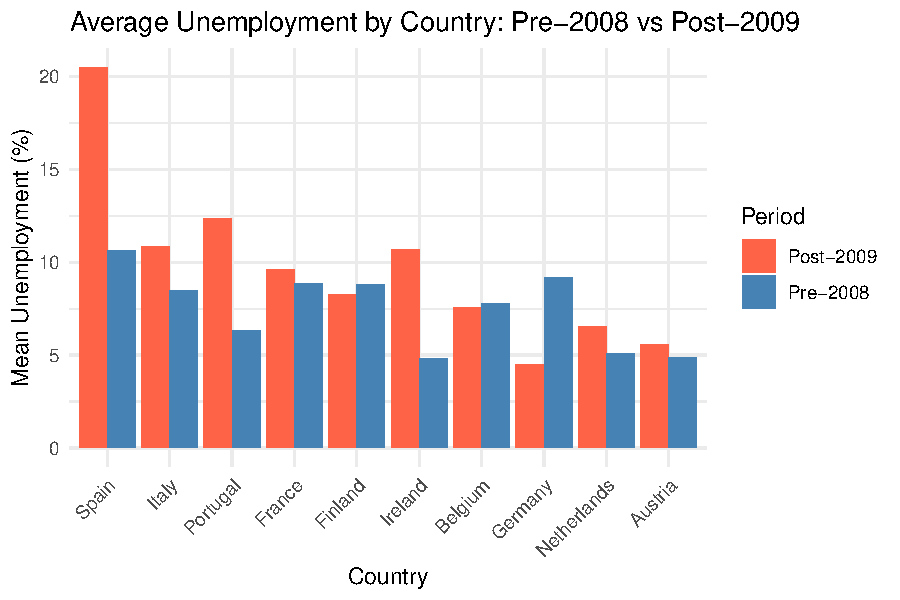
\includegraphics[width=\linewidth]{Average Unemployment by Country_Pre-2008 vs Post-2009.pdf}
        \caption{}
        \label{fig:unemployment}
    \end{subfigure}
    \hfill
    \begin{subfigure}{0.45\textwidth}
        \centering
        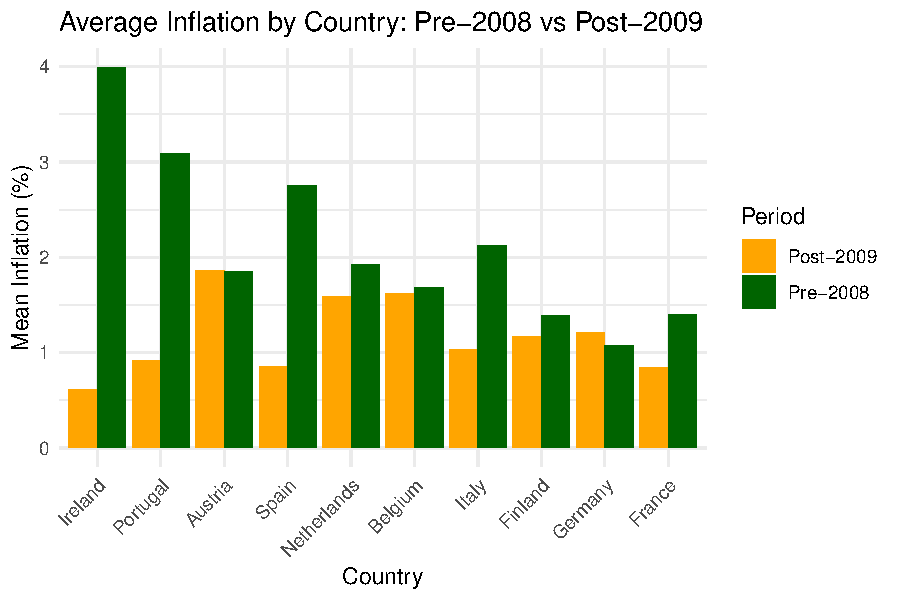
\includegraphics[width=\linewidth]{Average Inflation by Country_Pre-2008 vs Post-2009.pdf}
        \caption{}
        \label{fig:inflation}
    \end{subfigure}

    \caption{Average inflation and unemployment comparison across countries over both periods}
    \label{fig2:combined}
\end{figure}


Figure 2 left side suggests that in most countries unemployment has risen on average post crisis. There are few explanations to this change: Demand shock – banks were tightening lending, risk accelerating possible profits, household chose to spend less, taking less loans, saving more which lead to weak demand and lower output from supply side needing less employment to produce; Fiscal austerity to not fall into even bigger deficits by more peripheral countries (Spain and Portugal), governments cutting spending which weakened demand even more, not letting it build back up after a crisis; Hysteresis, a phenomenon when history impacts the state of the system – skills of longer unemployed people deteriorate and they have less and less chance of finding job later on. In construction heavy economies (Ireland, Portugal, Spain) construction employment collapsed after 2008 crisis, people in this sector having difficulties reallocating. Germany is a clear outlier, their post-2009 unemployment much lower than pre-crisis period. Germany planted Kurzabeit (short-time work) that let people stay in labour market with less hours instead of layoffs and government subsidizing wages (skills did not deteriorate during unemployed time, demand did not go down); Hartz reforms; High export country benefiting from growing demand in the world, especially in Asia and USA (not the case for Spain or Portugal). 

Right side displays another trend in inflation falling on average post-crisis. It is explained by similar facts: Demand shock results in firms not being able to raise prices and slower inflation; Internal devaluation – countries like Spain and Portugal had to cut wages to restore competitiveness, which led to less spending. ECB policy was too restraining, slower to do QE, raised interest rates in 2011, which did not help to encourage spending. Germany did not follow the trend due to reasons highlighted before.

\section{Analysis of correlations}

\begin{table}[H]
\centering
\caption{\label{tab:tab:correl}Correlation Between Inflation and Unemployment by Country and Period}
\centering
\begin{tabular}[t]{lc>{}c|cc}
\toprule
\multicolumn{1}{c}{ } & \multicolumn{2}{c}{Full Sample} & \multicolumn{2}{c}{By Period} \\
\cmidrule(l{3pt}r{3pt}){2-3} \cmidrule(l{3pt}r{3pt}){4-5}
Country & Full Sample & Excl. 2008-2009 & Pre-2008 & Post-2009\\
\midrule
Austria & -0.347 & -0.246 & -0.007 & -0.625\\
Belgium & -0.159 & -0.158 & -0.292 & -0.081\\
Finland & -0.232 & -0.090 & -0.100 & -0.198\\
France & -0.596 & -0.591 & -0.579 & -0.262\\
Germany & -0.242 & -0.254 & -0.093 & -0.633\\
\addlinespace
Ireland & -0.609 & -0.577 & -0.520 & -0.014\\
Italy & -0.596 & -0.588 & 0.316 & -0.546\\
Netherlands & -0.424 & -0.427 & -0.718 & 0.126\\
Portugal & -0.624 & -0.620 & -0.394 & 0.069\\
Spain & -0.761 & -0.764 & 0.053 & -0.099\\
\bottomrule
\end{tabular}
\end{table}

Overall, all countries were showing a degree of negative relationship between inflation and unemployment, as predicted by Phillips Curve. The strongest relationships are in Ireland, Portugal, and Spain, the volatility of the economy making Phillips Curve more prominent. Belgium is on the other end of the spectrum, with very weak relationship. The reason might be automatic wage indexation – when inflation goes up, wages are rising together, spiraling the inflation up, however, it is not an effect from unemployment shrinking, breaking the relationship; Generous unemployment benefits that does not let demand collapse, despite higher unemployment inflation stays high;

The fact that divided into two periods correlations are weaker then pulled together might confuse the reader until we learn about aggregation bias.

If we investigate pre-and-post crisis periods we notice that in most cases Phillips Curve has weakened. ECB policy regulates interest rates, inflation less tied to domestic conditions; Inflation expectations become anchored around 1\%, reacting to unemployment less; Hysteresis is known to make wages sticky at a new baseline level – employed workers, holding more bargaining power are bargaining for higher wages, which crowds out long-unemployed. So, despite long term unemployment, wages do not fall, inflation not going down.  

Countries that show only strengthening relationship after crisis are Germany, Austria, and Italy. Germany, as already mentioned, was undergoing reforms pre-2008, policy decoupled inflation from unemployment. Post-2009 economy reaped the benefits of previous policies and their need in monetary policy matched ECB; it was effective for Germany. 

For robustness check, we see that sample with excluded 2008-2009 yields very similar results, just Austria and Finland see a drop in correlation towards zero.


\section{Analysis of regression results}


\begin{table}[H]
\centering
\caption{Phillips Curve Results: Full Sample and Subsamples}
\label{tab:phillips_combined}

\begin{minipage}[t]{0.48\textwidth}
\centering
\scalebox{0.55}{%
\begin{tabular}{lcccc}
\\[-1.8ex]\hline\hline\\[-1.8ex]
 & \multicolumn{4}{c}{\textit{Dependent variable: Inflation}} \\
\cline{2-5}
\\[-1.8ex]
 & Model 1 & Model 2 & Model 3 & Model 4 \\
\\[-1.8ex] & (1) & (2) & (3) & (4) \\
\hline\\[-1.8ex]

\multicolumn{5}{l}{\textbf{Panel A: Full Sample (1999--2019)}} \\
\hline\\[-1.8ex]
Unemployment        & $-$0.191$^{***}$ & $-$0.180$^{***}$ &                  &                  \\
                    & (0.047)          & (0.055)          &                  &                  \\
Unemployment Gap    &                  &                  & $-$0.356$^{**}$  & $-$0.277$^{**}$  \\
                    &                  &                  & (0.177)          & (0.124)          \\
Trade Union Density &                  & $-$0.011         & $-$0.028         & $-$0.024         \\
                    &                  & (0.041)          & (0.050)          & (0.032)          \\
Globalisation       &                  & 0.007            & 0.031$^{**}$     & 0.019$^{*}$      \\
                    &                  & (0.007)          & (0.014)          & (0.011)          \\
Lagged Inflation    &                  &                  &                  & 0.366$^{***}$    \\
                    &                  &                  &                  & (0.049)          \\
\hline\\[-1.8ex]
Observations     & 840   & 840   & 840   & 840   \\
R$^{2}$          & 0.244 & 0.247 & 0.118 & 0.241 \\
Adjusted R$^{2}$ & 0.150 & 0.151 & 0.005 & 0.143 \\

\hline\\[-1.8ex]
\multicolumn{5}{l}{\textbf{Panel B: Excluding 2008--2009}} \\
\hline\\[-1.8ex]
Unemployment        & $-$0.131$^{***}$ & $-$0.119$^{***}$ &                  &                  \\
                    & (0.034)          & (0.044)          &                  &                  \\
Unemployment Gap    &                  &                  & $-$0.336$^{**}$  & $-$0.331$^{***}$ \\
                    &                  &                  & (0.166)          & (0.122)          \\
Trade Union Density &                  & 0.012            & 0.015            & 0.007            \\
                    &                  & (0.013)          & (0.014)          & (0.007)          \\
Globalisation       &                  & 0.008            & 0.026$^{**}$     & 0.012$^{***}$    \\
                    &                  & (0.010)          & (0.011)          & (0.004)          \\
Lagged Inflation    &                  &                  &                  & 0.496$^{***}$    \\
                    &                  &                  &                  & (0.043)          \\
\hline\\[-1.8ex]
Observations     & 760      & 760      & 760      & 760      \\
R$^{2}$          & 0.143    & 0.160    & 0.134    & 0.404    \\
Adjusted R$^{2}$ & 0.024    & 0.039    & 0.010    & 0.318    \\
\hline\hline\\[-1.8ex]
\end{tabular}}
\end{minipage}
\hfill
\begin{minipage}[t]{0.48\textwidth}
\centering
\scalebox{0.55}{%
\begin{tabular}{lcccc}
\\[-1.8ex]\hline\hline\\[-1.8ex]
 & \multicolumn{4}{c}{\textit{Dependent variable: Inflation}} \\
\cline{2-5}
\\[-1.8ex]
 & Model 1 & Model 2 & Model 3 & Model 4 \\
\\[-1.8ex] & (1) & (2) & (3) & (4) \\
\hline\\[-1.8ex]

\multicolumn{5}{l}{\textbf{Panel C: Subsample 1999--2007}} \\
\hline\\[-1.8ex]
Unemployment        & $-$0.204$^{***}$ & $-$0.198$^{***}$ &                  &                  \\
                    & (0.053)          & (0.040)          &                  &                  \\
Unemployment Gap    &                  &                  & $-$0.407         & $-$0.452$^{**}$  \\
                    &                  &                  & (0.255)          & (0.228)          \\
Trade Union Density &                  & 0.004            & 0.003            & $-$0.001         \\
                    &                  & (0.006)          & (0.007)          & (0.003)          \\
Globalisation       &                  & 0.017            & 0.037            & 0.016            \\
                    &                  & (0.036)          & (0.039)          & (0.022)          \\
Lagged Inflation    &                  &                  &                  & 0.501$^{***}$    \\
                    &                  &                  &                  & (0.079)          \\
\hline\\[-1.8ex]
Observations     & 360      & 360      & 360      & 360   \\
R$^{2}$          & 0.115    & 0.122    & 0.083    & 0.316 \\
Adjusted R$^{2}$ & $-$0.172 & $-$0.171 & $-$0.224 & 0.083 \\

\hline\\[-1.8ex]
\multicolumn{5}{l}{\textbf{Panel D: Subsample 2010--2019}} \\
\hline\\[-1.8ex]
Unemployment        & $-$0.046$^{*}$   & $-$0.066$^{***}$ &                  &                  \\
                    & (0.027)          & (0.025)          &                  &                  \\
Unemployment Gap    &                  &                  & $-$0.281$^{***}$ & $-$0.268$^{***}$ \\
                    &                  &                  & (0.093)          & (0.070)          \\
Trade Union Density &                  & $-$0.0003        & 0.0005           & 0.001            \\
                    &                  & (0.005)          & (0.005)          & (0.003)          \\
Globalisation       &                  & $-$0.010         & 0.001            & 0.0004           \\
                    &                  & (0.007)          & (0.010)          & (0.007)          \\
Lagged Inflation    &                  &                  &                  & 0.267$^{***}$    \\
                    &                  &                  &                  & (0.043)          \\
\hline\\[-1.8ex]
Observations     & 400      & 400      & 400      & 400      \\
R$^{2}$          & 0.061    & 0.081    & 0.074    & 0.202    \\
Adjusted R$^{2}$ & $-$0.205 & $-$0.187 & $-$0.196 & $-$0.034 \\
\hline\hline\\[-1.8ex]
\end{tabular}}
\end{minipage}

\vspace{4pt}
{\footnotesize\textit{Note:} Standard errors in parentheses (two-way clustered by country and quarter). $^{*}$p$<$0.1; $^{**}$p$<$0.05; $^{***}$p$<$0.01}
\end{table}


We present results from all regresssions and all samples and subsamples. When talking about results, we will call by letter the panel sample and by number next to it the regression model we are analyzing at that point.

A1: When we regress inflation on just unemployment we get negative statistically significant result, consistent with the main hypothesis. One percentage point increase in unemployment relative to its own average and relative to other countries at that time is associated with inflation going down by on average 0.19 percentage point. 

A2: We use regression two with controls. Unemployment is again negatively significant and the coefficient is almost the same as in first regression. This could suggest that our control variables are not the best as they do not help explain relation between inflation and unemployment. This is even more clear when looking at R squared which does not increase much. One of the reasons why this happens is our usage of two-way fixed effects. Trade union density does not change much over time, so when we are removing time invariant variables, we are essentially removing the effect of this variable. Despite globalisation changing from 1999 to 2019 more it still does not produce any statistically significant results; this  might be because globalisation was changing in Eurozone on a similar rate, on upward sloping trend. 

A3: Instead of Unemployment we will be using Unemployment gap now which we contruct by subtracting HP filter constructed NAIRU proxy from actual unemployment at that time period. Our model suggests that Unemployment gap coefficient is -0.36 and is significant at 5\% significance. When unemployment is above countries’ natural level by one percentage point it might indicate that inflation will fall on average by 0.36 percentage points. 

A4: We add lagged inflation into the model that works on average in a comparable way as expected future inflation. Unemployment gap is significant at 5\% level but is smaller in magnitude than before, coefficient is equal to -0.277. As we include the omitted variable of lagged inflation, it no longer picks up inflation persistence. Still the relation we found is consistent with our main hypothesis. Newly introduced lagged inflation is positive and significant, which is expected working through two channels – anchored expectations and how they impact spending/saving decisions and sticky prices (Taylor, 1977).  

We see that when introducing Unemployment Gap instead of Unemployment rate our R squared adjusted drops significantly. This might be an issue of constructed NAIRU – gap becomes noisy due to lack of information on NAIRU, especially after hysteresis after 2009.  

C1 and D1 comparison: Pre-crisis coefficient is more negative and statistically significant than post-crisis, which indicated that before crisis there was stronger relationship between unemployment and inflation.

C2 and D2 comparison: Both unemployment rates are significant, but unemployment magnitude of effect is measured to be stronger in pre-crisis times even when adding controls, which are insignificant in both models.

C3 and D3 comparison: Unemployment gap is insignificant in pre-crisis subsample. When we remove eurozone effects on countries we might be stripped of variation to have more significant results. Noisy regressor might also mess the inference. We cannot compare two models. 

C4 and D4 comparison: Unemployment gaps and lagged inflation are both significant. Comparing the coefficients on unemployment gaps we can see that pre-crisis is associated with more negative effect of change of countries’ average level of unemployment gap. This is also consistent with our secondary hypothesis that Phillips Curve flattened after the crisis. Additionally, lagged inflation is more positive in pre-crisis period than post-crisis. It might indicate that after crisis, inflation expectations were anchored by the ECB. Also, it could be that firms and households rely more on past inflation when forming expectations. 

Both panel C and panel D showcase negative adjusted R squared in most scenarios. This might happen due to little variation after TWFE especially after separating two periods, leaving less variation with the same number of parameters.  

In general, more complex regressions (3 and 4) find stronger relation between unemployment and inflation. Also, post crisis relation is smaller, but including NAIRU and inflation expectations increases statistical significance of the relation. On top of that R squared increases. This is consistent with our additional hypothesis that Augmented Phillips Curve might better explain post crisis period relation. 
However, our analysis suffers from some issues such as Nickell Bias. Since the fourth model includes lagged dependent variable, there is a mechanical correlation between the demeaned error and demeaned lagged dependent variable. It does decrease the credibility of the fourth model, however our sample sizes and time dimension is quite large, therefore the issue is not so big. That is why the 3rd and 4th models are likely to be the best for answering our main research question while the previous regressions are more for robustness and comparison. There is a case to be made for TWFE taking away a lot of variation which causes R squared to be very low. But, explaining all variation in inflation is not our objective — isolating the specific within-country, over-time relationship between unemployment and inflation is. Also, 2008-2009 excluded sample does not show big differences from the full sample, so our robustness check passes.

\section{Conclusion}

Our report analyzed the relation between unemployment and inflation using panel data from Eurozone countries and using Two-way fixed effects regressions.

In all four models, we find that for the full sample, selected Eurozone countries experience negative statistically significant relation between unemployment and inflation ranging from 0.18 to 0.35 percentage point decrease in inflation when unemployment rate goes up by 1 percentage point consistent with Hazell(2022), Ball(2021). Therefore our main hypothesis seems to hold.

More complex models including NAIRU and inflation expectations produce steeper estimates, though introduced biases prevent a conclusive comparison with simpler specifications.


Subsample analysis shows that post financial crisis, the negative relation between unemployment and inflation weakened across all models (from -0.45 to -0.27 in model 4). This is consistent with our hypothesis that Phillips curve flattened and previous research that found changing relation post events like 1970s energy crisis or 2008-09 great recession  (Blanchard, 2015), (Ball, 2011). Further research needs to be done to understand why the Phillips curve is susceptible to change after economic shocks.

A statistically significant beta with low R squared we get in our regressions means unemployment does matter for inflation, but there is substantial unexplained noise. This is consistent with the literature that the Phillips curve is a weak but real relationship, especially post-2000 (Ball, 2011). 

Limitations of our model include using lagged dependent variable. However we are not able to find better alternative without going into complications for this limited research report. Secondly, we might be using wrong functional form regressions as the relation between unemployment and inflation could be non-linear. What is more, estimating NAIRU using HP filter brings uncertainty and bias. We might also lack some additional and better explanatory control variables. Due to all these drawbacks, our estimation and conclusions are only descriptive. We lack identifying assumption to make causal inference.

Finally, in more recent times, central bank trying to operate optimally, will seek to increase inflation when output is below potential, causing simultaneity bias between inflation and unemployment. Therefore,  flattening of the Phillips Curve in Eurozone may partly reflect successful monetary policy of ECB rather than the disappearance of the inflation–output relationship (McLeay, 2019).




\begin{thebibliography}{00}

%% For authoryear reference style
%% \bibitem[Author(year)]{label}
%% Text of bibliographic item

\bibitem[Ball and Mazumder(2011)]{ball2011great}
Ball, L., \& Mazumder, S. (2011). Inflation dynamics and the Great Recession. \textit{Brookings Papers on Economic Activity}, 337--405.

\bibitem[Ball and Mazumder(2021)]{ball2021phillips}
Ball, L., \& Mazumder, S. (2021). A Phillips curve for the euro area. \textit{International Finance}, \textit{24}, 2--17. 

\bibitem[Gordon(2011)]{gordon2011history}
Gordon, R. J. (2011). The history of the Phillips curve: Consensus and bifurcation. \textit{Economica}, \textit{78}, 10--50. 

\bibitem[Hazell et al.(2022)]{hazell2020slope}
Hazell, J., Herreño, J., Nakamura, E., \& Steinsson, J. (2020). \textit{The slope of the Phillips curve: Evidence from U.S. states} (NBER Working Paper No. 28005). 

\bibitem[Del Negro et al.(2020)]{delnegro2020phillips}
Del Negro, M., Lenza, M., Primiceri, G. E., \& Tambalotti, A. (2020). \textit{What's up with the Phillips curve?} (NBER Working Paper No. 27003). 

\bibitem[Phillips(1958)]{phillips1958relation}
Phillips, A. W. (1958). The relation between unemployment and the rate of change of money wage rates in the United Kingdom, 1861--1957. \textit{Economica}, 283--299.

\bibitem[Woodcock(2020)]{woodcock2020hartz}
Woodcock, S. D. (2020). \textit{The effect of the Hartz labor market reforms on post-unemployment wages, sorting, and matching} (IZA Discussion Paper No. 13300).

\bibitem[Gygli et al.(2019)]{gygli2019kof}
Gygli, S., Haelg, F., Potrafke, N., \& Sturm, J.-E. (2019). The KOF Globalisation Index -- Revisited. \textit{Review of International Organizations}, \textit{14}(3), 543--574. 

\bibitem[Dreher(2006)]{dreher2006globalization}
Dreher, A. (2006). Does globalization affect growth? Evidence from a new index of globalization. \textit{Applied Economics}, \textit{38}(10), 1091--1110.

\bibitem[Cameron et al.(2011)]{cameron2011robust}
Cameron, A. C., Gelbach, J. B., \& Miller, D. L. (2011). Robust inference with multiway clustering. \textit{Journal of Business \& Economic Statistics}, \textit{29}(2), 238--249.

\bibitem[Phelps and Taylor(1977)]{phelps1977stabilizing}
Phelps, E. S., \& Taylor, J. B. (1977). Stabilizing powers of monetary policy under rational expectations. \textit{Journal of Political Economy}, \textit{85}(1), 163--190.

\bibitem[McLeay and Tenreyro(2019)]{mcleay2019optimal}
McLeay, M., \& Tenreyro, S. (2019). Optimal inflation and the identification of the Phillips curve. \textit{NBER Macroeconomics Annual}, \textit{34}, 199--255. 

\bibitem[Blanchard et al.(2015)]{blanchard2015inflation}
Blanchard, O., Cerutti, E., \& Summers, L. (2015). \textit{Inflation and activity -- Two explorations and their monetary policy implications} (IMF Working Paper No. 15/230). International Monetary Fund.

\bibitem[Ball and Mazumder(2019)]{ball2019anchored}
Ball, L., \& Mazumder, S. (2019). A Phillips curve with anchored expectations and short-term unemployment. \textit{Journal of Money, Credit and Banking}, \textit{51}(1), 111--137.

\bibitem[Friedman(1968)]{friedman1968role}
Friedman, M. (1968). The role of monetary policy. \textit{American Economic Review}, \textit{58}(1), 1--17.

\bibitem[Roberts(1995)]{roberts1995new}
Roberts, J. M. (1995). New Keynesian economics and the Phillips curve. \textit{Journal of Money, Credit and Banking}, \textit{27}(4), 975--984.

\bibitem[Galí and Gertler(1999)]{gali1999inflation}
Gal\'{\i}, J., \& Gertler, M. (1999). Inflation dynamics: A structural econometric analysis. \textit{Journal of Monetary Economics}, \textit{44}(2), 195--222.

\bibitem[Galí et al.(2001)]{gali2001european}
Gal\'{\i}, J., Gertler, M., \& L\'opez-Salido, D. (2001). European inflation dynamics. \textit{European Economic Review}, \textit{45}(7), 1237--1270.

\bibitem[IMF(2023)]{imf2023ireland}
International Monetary Fund, European Department. (2023). \textit{Boom without disease? Impact of multinational enterprises in Ireland}. International Monetary Fund. eISBN: 9798400261428.


\bibitem[Costain et al.(2010)]{costain2010employment}
Costain, J., Jimeno, J. F., \& Thomas, C. (2010). \textit{Employment fluctuations in a dual labor market} (Working Paper No. 1013). Banco de Espa\~na.

\bibitem[Santos and Fernandes(2015)]{santos2015portugal}
Santos, A. B., \& Fernandes, S. (2015). \textit{Internal devaluation and unemployment: The case of Portugal}. ISCTE -- University Institute of Lisbon; Jacques Delors Institute.



\end{thebibliography}

\appendix


\section{}

\begin{itemize}
    \item $\pi_{it,q}$ = inflation for country $i$ in quarter $q$ of year $t$
    \item $u_{it,q}$ = unemployment rate for country $i$ in quarter $q$ of year $t$
    \item $(u_{it,q} - u^{*}_{it,q})$ = unemployment gap; actual unemployment minus NAIRU for country $i$ in quarter $q$ of year $t$
    \item $u^{*}_{it,q}$ = NAIRU (Non-Accelerating Inflation Rate of Unemployment)
    \item $\pi^{e}_{it,q}$ = inflation expectations (lagged inflation from one year before)
    \item $X_{it,q}$ = controls (effect that are time varying and specific to a country)
    \item $\mu_{i}$ = country fixed effects
    \item $\lambda_{t,q}$ = time fixed effects
    \item $\varepsilon_{it,q}$ = error term
\end{itemize}


\end{document}




\endinput
%%
%% End of file `elsarticle-template-harv.tex'.


